% Options for packages loaded elsewhere
\PassOptionsToPackage{unicode}{hyperref}
\PassOptionsToPackage{hyphens}{url}
%
\documentclass[
  12pt,
  a4paper]{extarticle}
\title{Analysis 1B --- Tutorial 4}
\author{Christian Jones: University of Bath}
\date{February 2023}

\usepackage{amsmath,amssymb}
\usepackage{lmodern}
\usepackage{iftex}
\ifPDFTeX
  \usepackage[T1]{fontenc}
  \usepackage[utf8]{inputenc}
  \usepackage{textcomp} % provide euro and other symbols
\else % if luatex or xetex
  \usepackage{unicode-math}
  \defaultfontfeatures{Scale=MatchLowercase}
  \defaultfontfeatures[\rmfamily]{Ligatures=TeX,Scale=1}
\fi
% Use upquote if available, for straight quotes in verbatim environments
\IfFileExists{upquote.sty}{\usepackage{upquote}}{}
\IfFileExists{microtype.sty}{% use microtype if available
  \usepackage[]{microtype}
  \UseMicrotypeSet[protrusion]{basicmath} % disable protrusion for tt fonts
}{}
\makeatletter
\@ifundefined{KOMAClassName}{% if non-KOMA class
  \IfFileExists{parskip.sty}{%
    \usepackage{parskip}
  }{% else
    \setlength{\parindent}{0pt}
    \setlength{\parskip}{6pt plus 2pt minus 1pt}}
}{% if KOMA class
  \KOMAoptions{parskip=half}}
\makeatother
\usepackage{xcolor}
\IfFileExists{xurl.sty}{\usepackage{xurl}}{} % add URL line breaks if available
\IfFileExists{bookmark.sty}{\usepackage{bookmark}}{\usepackage{hyperref}}
\hypersetup{
  pdftitle={Analysis 1B --- Tutorial 4},
  pdfauthor={Christian Jones: University of Bath},
  hidelinks,
  pdfcreator={LaTeX via pandoc}}
\urlstyle{same} % disable monospaced font for URLs
\usepackage[margin=2.5cm]{geometry}
\usepackage{longtable,booktabs,array}
\usepackage{calc} % for calculating minipage widths
% Correct order of tables after \paragraph or \subparagraph
\usepackage{etoolbox}
\makeatletter
\patchcmd\longtable{\par}{\if@noskipsec\mbox{}\fi\par}{}{}
\makeatother
% Allow footnotes in longtable head/foot
\IfFileExists{footnotehyper.sty}{\usepackage{footnotehyper}}{\usepackage{footnote}}
\makesavenoteenv{longtable}
\usepackage{graphicx}
\makeatletter
\def\maxwidth{\ifdim\Gin@nat@width>\linewidth\linewidth\else\Gin@nat@width\fi}
\def\maxheight{\ifdim\Gin@nat@height>\textheight\textheight\else\Gin@nat@height\fi}
\makeatother
% Scale images if necessary, so that they will not overflow the page
% margins by default, and it is still possible to overwrite the defaults
% using explicit options in \includegraphics[width, height, ...]{}
\setkeys{Gin}{width=\maxwidth,height=\maxheight,keepaspectratio}
% Set default figure placement to htbp
\makeatletter
\def\fps@figure{htbp}
\makeatother
\setlength{\emergencystretch}{3em} % prevent overfull lines
\providecommand{\tightlist}{%
  \setlength{\itemsep}{0pt}\setlength{\parskip}{0pt}}
\setcounter{secnumdepth}{5}
\newcommand{\BOO}{BOO}
\usepackage {hyperref}
\hypersetup {colorlinks = true, linkcolor = blue, urlcolor = blue}
\usepackage{float}
\ifLuaTeX
  \usepackage{selnolig}  % disable illegal ligatures
\fi

\usepackage{amsthm}
\theoremstyle{plain}
\newtheorem*{theorem*}{Theorem}\newtheorem{theorem}{Theorem}[section]
\theoremstyle{definition}
\newtheorem*{definition*}{Definition}\newtheorem{definition}{Definition}[section]
\theoremstyle{plain}
\newtheorem*{proposition*}{Proposition}\newtheorem{proposition}[theorem]{Proposition}
\newtheorem*{Definitions*}{Definitions}\newtheorem{Definitions}[definition]{Definitions}
\theoremstyle{plain}
\newtheorem*{lemma*}{Lemma}\newtheorem{lemma}{Lemma}[section]
\theoremstyle{plain}
\newtheorem*{corollary*}{Corollary}\newtheorem{corollary}{Corollary}[section]
\theoremstyle{plain}
\newtheorem*{conjecture*}{Conjecture}\newtheorem{conjecture}{Conjecture}[section]
\theoremstyle{definition}
\newtheorem*{example*}{Example}\newtheorem{example}{Example}[section]
\theoremstyle{definition}
\newtheorem*{exercise*}{Exercise}\newtheorem{exercise}{Exercise}[section]
\newtheorem*{Thought*}{Thought}\newtheorem{Thought}{Thought}[section]
\theoremstyle{remark}
\newtheorem*{remark*}{Remark}
\newtheorem*{solution*}{Solution}
\newtheorem*{Example*}{Example}
\theoremstyle{remark}
\newtheorem*{Proof*}{Proof}
\newtheorem*{Examples*}{Examples}
\let\BeginKnitrBlock\begin \let\EndKnitrBlock\end


%\usepackage[english,shorthands=off]{babel}
\usepackage{etoolbox}
\usepackage{spverbatim}
\makeatletter
\@ifpackageloaded{float}{}{\usepackage{float}}
\@ifpackageloaded{adjustbox}{}{\usepackage[Export]{adjustbox}}
\makeatother
\floatplacement{figure}{H}
\newcommand{\scalefactor}{1.2}
\adjustboxset*{min width=\scalefactor\width,max width=\linewidth}
\renewcommand{\familydefault}{phv}
\fontfamily{phv}\selectfont
\renewcommand{\em}{\bf}\renewcommand{\textit}{\textbf}\renewcommand{\emph}{\textbf}\renewcommand{\it}{\bf}\renewcommand{\itshape}{\bf}
\setlength{\parindent}{0.0pt}
\setlength{\parskip}{1.0\baselineskip}
\renewcommand{\baselinestretch}{1.5}\selectfont
\setlength{\mathsurround}{0.2em}
\setlength{\arraycolsep}{0.5cm}\renewcommand{\arraystretch}{1.5}
\addtolength{\jot}{\baselineskip}
\renewcommand{\;}{\,}
\sloppy
\allowdisplaybreaks
\usepackage{amsthm}
\newtheoremstyle{plain}{20pt}{3pt}{}{}{\bfseries}{.\newline\nobreak}{1.0em\nobreak}{}
\newtheoremstyle{definition}{20pt}{3pt}{}{}{\bfseries}{.\newline\nobreak}{1.0em\nobreak}{}
\newtheoremstyle{remark}{20pt}{3pt}{}{}{\bfseries}{.\newline\nobreak}{1.0em\nobreak}{}
\csundef{Proof}
\csundef{endProof}
\newenvironment{Proof}
  {\noindent{\bf Proof.}\hspace*{1em}}% Begin
  {\qed\par}% End
%% When redefining an environment it is vital that it has 
%% the same number of arguments as the original
\renewenvironment{proof}[1][\proofname]
  {\trivlist\item\relax\noindent{\bf {#1}.}\hspace*{1em}}% Begin
  {\qed\endtrivlist}% End

\begin{document}
\maketitle

{
\setcounter{tocdepth}{2}
\tableofcontents
}
\newpage
\pagenumbering{arabic}

\hypertarget{introduction}{%
\section*{Introduction}\label{introduction}}
\addcontentsline{toc}{section}{Introduction}

Here is the material to accompany the 4th Analysis 1B Tutorial on the 27th February. Alternative formats can be downloaded by clicking the download icon at the top of the page. Please send any comments or corrections to \href{mailto:caj50@bath.ac.uk}{Christian Jones (caj50)}. To return to the homepage, click \href{http://caj50.github.io/tutoring.html}{here}.

\hypertarget{lecture-recap}{%
\section{Lecture Recap}\label{lecture-recap}}

\hypertarget{sequential-continuity}{%
\subsection{Sequential Continuity}\label{sequential-continuity}}

Recall the definition of function continuity from last week:
\BeginKnitrBlock{definition}[Continuity]
{\label{def:def1} }Let \(D \subseteq \mathbb{R}\), and \(f: D \to \mathbb{R}\). Then \(f\) is continuous at a point \(c\) if \[\forall \epsilon > 0\;\;\exists \delta > 0\;\;\text{s.t.}\;\;\forall x \in D,\;\; \lvert x - c \rvert < \delta \Rightarrow \lvert f(x) - f(c) \rvert < \epsilon.\]
\EndKnitrBlock{definition}
Much like we did with limits, we can characterise continuity in terms of sequences. A bit of déjà vu here is completely normal, as this is something that was covered in Semester 1:

\BeginKnitrBlock{definition}[Sequential Continuity]
{\label{def:def2} }Let \(D \subseteq \mathbb{R}\), and \(f: D \to \mathbb{R}\). Then \(f\) is sequentially continuous at a point \(c\) if for all sequences \((x_n)_n\) in \(D\) converging to \(c\), we have that \(\lim_{n \to \infty}f(x_n) = f(c).\)
\EndKnitrBlock{definition}

A comparison between the two definitions is seen in Figure \ref{fig:seqcnt}. Remarkably, we can show that these two definitions are equivalent to each other:

\BeginKnitrBlock{theorem}[Sequential Characterisation of Continuity]
{\label{thm:thm1} }Let \(D \subseteq \mathbb{R}\), and \(f: D \to \mathbb{R}\). Then \(f\) is continuous at a point \(c\) if and only if it is sequentially continuous at \(c\).
\EndKnitrBlock{theorem}
So why is this theorem useful? Basically, it says that you can use all the theory you learnt about sequences last semester to continuous functions. For example, last semester you showed that \(\sin\), \(cos\) and the exponential function \(\exp\) were sequentially continuous on \(\mathbb{R}\). Now you know they are continuous without doing any extra work! Also, this allows you to deduce the \emph{Intermediate Value Theorem} for continuous functions too --- see later for more details.

\begin{figure}
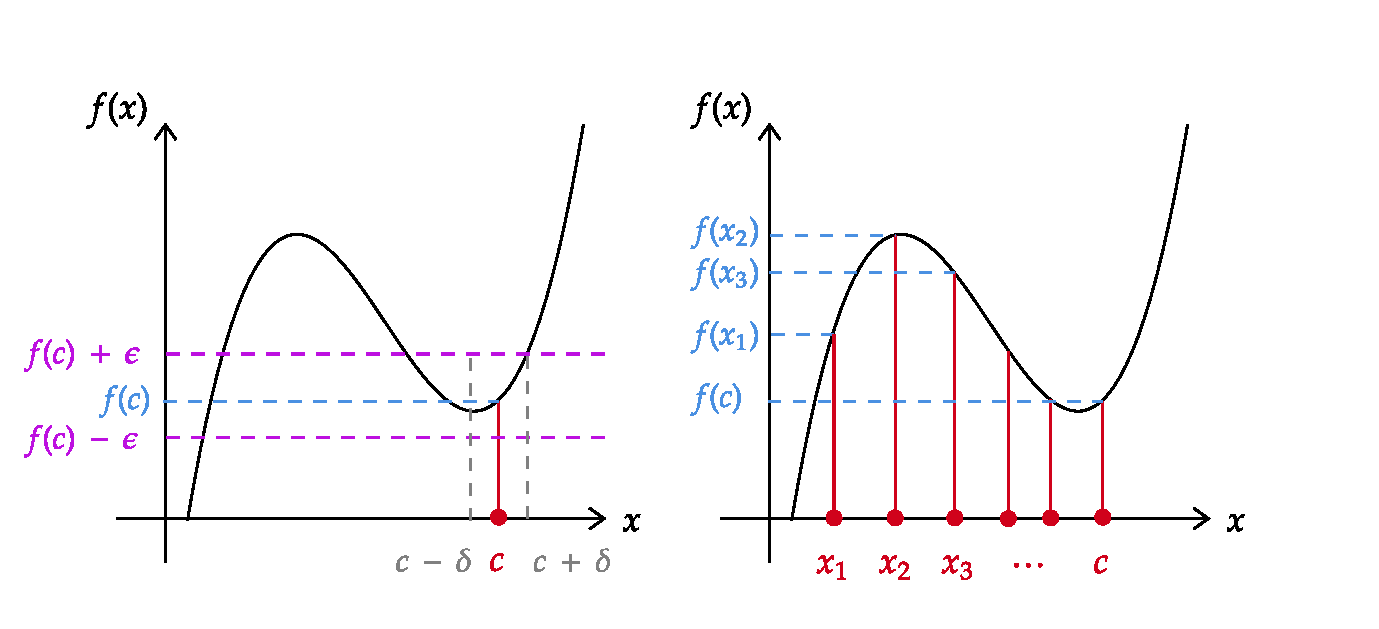
\includegraphics[width=\Width,height=\Height]{Sequential Continuity} \caption{A diagram illustrating the definitions of continuity at a point $c$ (left), and sequential continuity at a point $c$ (right), for a function $f$. It turns out that these definitions are completely equivalent!}\label{fig:seqcnt}
\end{figure}

Before we move on, Theorem \ref{thm:thm1} also gives us a way of proving that a function is \emph{not} continuous. We show this through Tutorial Question 2 on Problem Sheet 4.

\BeginKnitrBlock{example}
{\label{exm:ex1} }Let \(f:\mathbb{R} \to \mathbb{R}\) be defined by \[f(x) = \begin{cases}
1 \;\;\text{if}\;\;x\in\mathbb{Q},\\
0 \;\;\text{if}\;\;x\in\mathbb{R}\setminus\mathbb{Q}.\end{cases}\] Further, define \(h:\mathbb{R} \to \mathbb{R}\) by \(h(x) = xf(x)\). Determine all points where \(h\) is continuous.
\EndKnitrBlock{example}

\BeginKnitrBlock{solution*}
The main result of Tutorial Question 2 shows us that \(h\) is continuous at exactly one point --- zero.

To prove \(h\) is continuous at \(0\), fix \(\epsilon > 0\), and suppose \(\lvert x \rvert < \delta\) for some \(\delta > 0\) to be chosen later. Then
\begin{align*}
\lvert h(x) - h(0) \rvert = \lvert x f(x) \rvert \leq \lvert x \rvert < \delta.
\end{align*}
Hence, taking \(\delta = \epsilon\) gives that
\begin{align*}
\lvert x \rvert < \delta \Longrightarrow \lvert h(x) - h(0) \rvert < \epsilon.
\end{align*}
As \(\epsilon\) was arbitrary, we have shown \(h\) is continuous at \(0\).

To prove \(h\) is discontinuous everywhere else, fix \(c \in \mathbb{R}\setminus \lbrace 0 \rbrace.\) Since both the rational numbers (\(\mathbb{Q}\)) and irrational numbers (\(\mathbb{R}\setminus\mathbb{Q}\)) are dense in \(\mathbb{R}\), we can choose sequences \((x_n)_n\) and \((y_n)_n\) in \(\mathbb{R}\) such that

\begin{enumerate}
\def\labelenumi{\arabic{enumi}.}
\tightlist
\item
  \(\lim_{n \to \infty} x_n = c = \lim_{n \to \infty} y_n\),
\item
  \(x_n \in \mathbb{Q}\;\;\forall n \in \mathbb{N},\) and
\item
  \(y_n \in \mathbb{R}\setminus\mathbb{Q}\;\;\forall n \in \mathbb{N}.\)
\end{enumerate}

Now, \[h(x_n) = x_n f(x_n) = x_n \to c \;\;\text{as}\;\; n \to \infty,\] and \[h(y_n) = y_n f(y_n) = 0 \to 0 \;\;\text{as}\;\; n \to \infty.\] So, if \(c\) is rational, we have shown that \(h(y_n)\not\to h(c)\). If \(c\) is irrational, we have shown that \(h(x_n)\not\to h(c)\). Therefore, \(h\) cannot be continuous at \(c\) by Theorem \ref{thm:thm1}.
\EndKnitrBlock{solution*}

\textbf{Extension!}

\BeginKnitrBlock{example}
{\label{exm:ex2} }We can even use this example to produce a function defined on \(\mathbb{R}\) which is only continuous on \(\mathbb{Z}\)! Using the \(h\) from Example \ref{exm:ex1}, we can define \(k(x) = h(x)\) if \(x \in (-1/2, 1/2]\), and otherwise set \(k(x + 1) = k(x).\) This periodicity condition ensures that since \(h\) is only continuous at \(0\), \(k\) must be continuous only at each integer value.
\EndKnitrBlock{example}

\hypertarget{building-continuous-functions}{%
\subsection{Building Continuous Functions}\label{building-continuous-functions}}

Another thing that the sequential characterisation of continuity gives you is an `algebra of continuity'. In other words, continuous functions behave as you'd expect them to:

\BeginKnitrBlock{theorem}[Algebra of Continuity]
{\label{thm:thm2} }Let \(c, \lambda \in \mathbb{R}\), and let \(f,g: D \to \mathbb{R}\) Suppose \(f\) and \(g\) are continuous at \(c \in D\). Then the following functions are continuous at \(c\):

\begin{enumerate}
\def\labelenumi{\arabic{enumi}.}
\item
  \(f + g\).
\item
  \(\lambda f\)
\item
  \(fg\) (where \((fg)(x) = f(x)g(x)\))
\item
  \(\frac{f}{g}\) (when \(g(c) \neq 0.\))
\end{enumerate}
\EndKnitrBlock{theorem}

However, one thing that we can do with functions that we couldn't do with sequences is compose them. The following result tells us exactly when the composition \(f\circ g\) is continuous!

\BeginKnitrBlock{proposition}[Continuity of Composition]
{\label{prp:prop1} }Let \(f: D \to \mathbb{R}\) and \(g: E \to \mathbb{R}\), with \(g(x) \in D \;\; \forall x \in E.\) Then, if \(g\) is continuous at \(c \in E\), and \(f\) is continuous at \(g(c) \in D\), then the composition \(f\circ g : E \to \mathbb{R}\) is continuous at \(c\).
\EndKnitrBlock{proposition}
A similar statement for limits also holds, but in that case, the continuity of \(f\) is crucial --- see Problem Sheet 4 for more details!

\hypertarget{intermediate-value-theorem}{%
\subsection{Intermediate Value Theorem}\label{intermediate-value-theorem}}

Here's one of the main theorems from last semester!

\BeginKnitrBlock{theorem}[Intermediate Value Theorem (IVT)]
{\label{thm:thm3} }Suppose \(a,b \in \mathbb{R}\) with \(a < b\), and that \(f:[a,b] \to \mathbb{R}\) is continuous\footnote{If you like your notation, you can say that \(f \in C^0([a,b]),\) which is the set of continuous functions on \([a,b]\).}. Then, if \(y \in \mathbb{R}\) is such that \(f(a) \leq y \leq f(b)\), then \(\exists c \in [a,b]\) such that \(f(c) = y\).
\EndKnitrBlock{theorem}
Diagrammatically, we might be in a situation like in Figure \ref{fig:ivt}. Note that there may be more than one \(c\) that fulfills the conclusion of this theorem. Also, the theorem doesn't tell you what this \(c\) is; it only says that a \(c\) must exist.

\begin{figure}
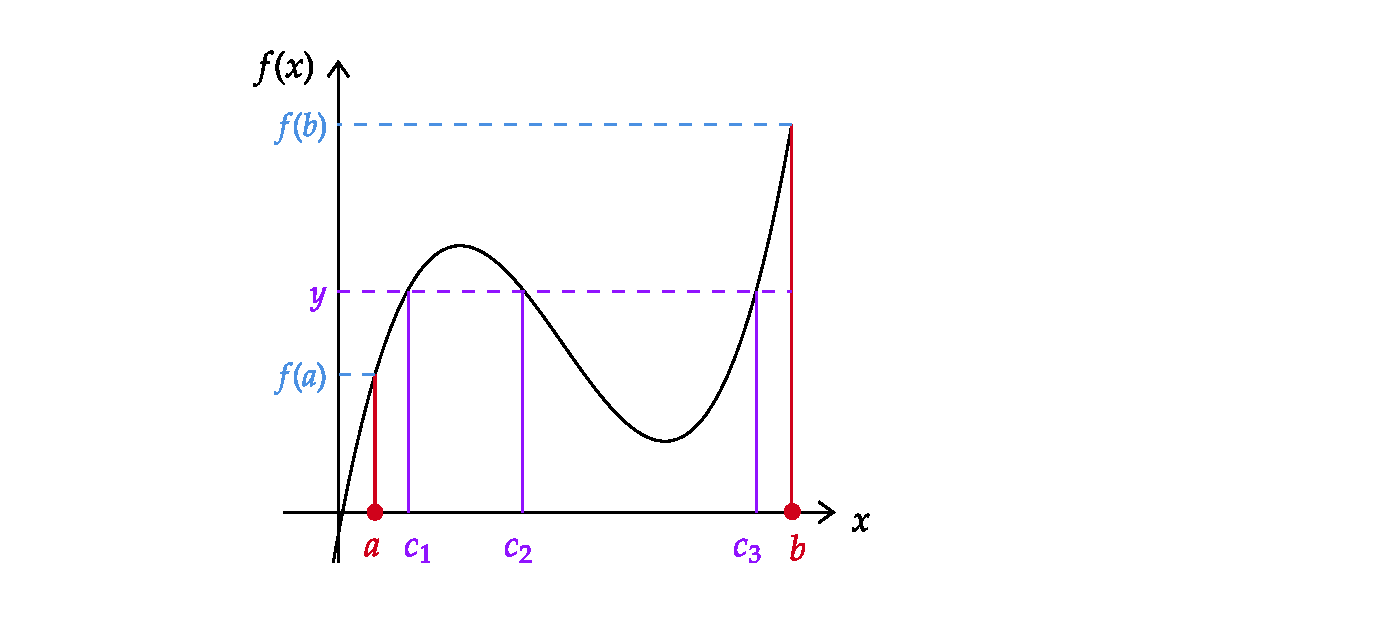
\includegraphics[width=\Width,height=\Height]{ivt} \caption{This function is continuous on $[a,b]$, and for $y$ as in the diagram, $y$ lies between $f(a)$ and $f(b)$. Hence the IVT applies, and so there exists $c$ in the interval $[a,b]$ such that $f(c)=y$. In this scenario, $c$ can be any one of $c_1,c_2$ or $c_3$.}\label{fig:ivt}
\end{figure}

The IVT is very good for proving existence of square roots (and roots of any degree!), proving that functions have zeros, and proving that at any given point in time, there exists two points on the equator with exactly the same temperature\footnote{On an idealised Earth, anyway.}.

\hypertarget{hints}{%
\section{Hints}\label{hints}}

As per usual, here's where you'll find the problem sheet hints!

\begin{enumerate}
\def\labelenumi{\arabic{enumi})}
\tightlist
\item
  These two examples are largely similar to the ones we did in tutorials (and I think there's a couple of examples in the lecture notes). Just make sure to explain fully why the function is/isn't continuous at a given point. And for once, there's no \(\epsilon-\delta\) argument in sight!
\item
  For this question, I'd recommend looking at `Problem Sheet Week 10' from last semester, if you want an example along these lines. In regards to your solution, make it explicit that all hypotheses of the IVT are satisfied!
\item
  For the first part (i.e.~proving the given result), use the sequential characterisation of limits and continuity. For the second part, try and find functions \(f,g: \mathbb{R} \to \mathbb{R}\) which satisfy
  \begin{align*}
  g(f(x)) = \begin{cases}
  1 \quad x\leq 0,\\
  0 \quad x > 0.
  \end{cases}
  \end{align*}
  \emph{(Googling `ramp function' might help with choosing one of \(f\) or \(g\).)}
\end{enumerate}

\end{document}
